\documentclass{article}
\usepackage[utf8]{inputenc}
\usepackage{tikz} %package for plots, graphics and functions

\title{Basic Shapes}
\author{Arman Daneshdoost}
\date{March 2024}

\begin{document}
	\maketitle
		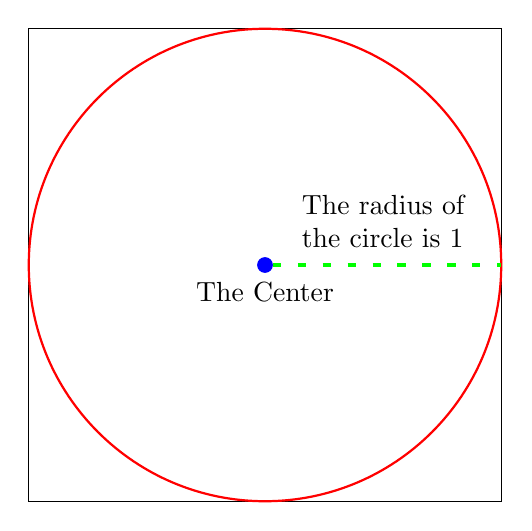
\begin{tikzpicture}
			\draw (-3, -3) rectangle(3, 3); %square with legth 3
			\draw [red, thick] (0, 0) circle[radius = 3];  %red circle with radius 3 on (0, 0) start point
			%\draw [fill, blue] (0, 0) circle [radius = 0.1]; %filled circle with radius 0.1
			\fill [blue] (0, 0) circle [radius = 0.1];
			\draw [green, loosely dashed, ultra thick] (0.1, 0) -- (3, 0); %we can have densely dotted or dashed
			
			\node[below] at (0, -0.1) {The Center}; %adding text on shapes - above or below or left and right
			
			\node[above, align=left] at (1.5, 0.1) {The radius of \\ the circle is 1}; %aligning the text in another line to left
		\end{tikzpicture}
		\section{Basic Shapes Exercises}
		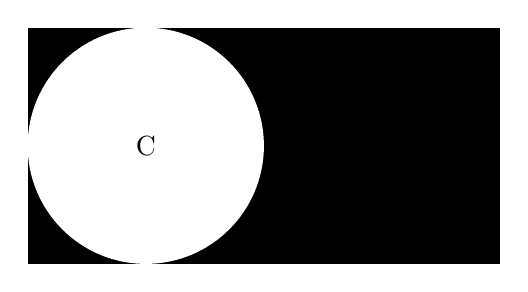
\begin{tikzpicture}
			\fill [black] (0, 0) rectangle(6, 3);
			\fill [white] (1.5, 1.5) circle [radius = 1.5];
			\node[centered] at (1.5, 1.5) {C};
		\end{tikzpicture}
\end{document}